\chapter{مقدمه}
بر اساس قانون مور
\LTRfootnote{Moore's law}
قدرت پردازنده های کامپیوتر های کلاسیک هر دو سال، دو برابر میشود. اما این رویه تا حدی ادامه خواهد داشت که محدودیت های دنیای فیزیک کلاسیک به آن اجازه دهند. چرا که اندازه ی اعضای تشکیل دهنده ی پردازنده ها به حدی کوچک میشود که ناخودآگاه وارد فضای کوچک کوانتوم
\LTRfootnote{Quantum}
 میشوند. پیشبینی میشود این اتفاق در سال 2050 رخ دهد.
\\
 پیچیدگی محاسباتی
\LTRfootnote{Computational complexity}
 برخی الگوریتم ها در کامپیوتر های کلاسیک کمتر قابلیت کاهش ندارند. در حالی که کامپیوتر های کوانتومی، در تئوری میتوانند با مقدار بزرگی داده همانند یک واحد داده برخورد کنند و پیچیدگی محاسباتی الگوریتم ها را کاهش دهند.
\cite{singhbook1in2}
به طور کلی، محاسبات کوانتومی از کنش و واکنش مواد در جهان در سطح ذرات تشکیل دهنده ی آن بهره میگیرد و بر روی بستر پدیده ی نسبیت خاص
\LTRfootnote{Special relativity}
 پایه‌گذاری شده‌است. 
\\
برای مثال، کامپیوتر کلاسیک مشکلی در پیدا کردن نام فرد موردنظر در یک کتاب تلفن ندارند. اما برای مسائل ریاضی بهینه سازی پیچیده
\LTRfootnote{Complex mathematical optimizing}
  که مسائلی هستند که برای پیدا کردن حالت بهینه با توجه به متغیر های مختلف است، کامپیوتر های کلاسیک پاسخگو نیستند. از جمله این مسائل میتوان به اختصاص دادن منابع در ساخت یک برج بزرگ برای بدست آوردن کمترین خرج ممکن اشاره کرد.  چنین مسائلی در همه ی خوزه ها وجود دارند و کامپیوتر های کوانتومی برای اجرای این الگوریتم ها بسیار مناسب هستند. 
\cite{singhbook1in4}

‌\section{‌خواص دنیای محاسبات کوانتومی}\label{sec1}
\subsection{کیوبیت}
کیوبیت ها
\LTRfootnote{Qubits}
 در کامپیوتر های کوانتومی، معادل بیت ها
\LTRfootnote{bits}
 در کامپیوتر های کلاسیک هستند. یک بیت یا در حالت صفر قرار دارد یا در حالت یک قرار دارد. تفاوت کیوبیت ها در این است که میتوانند حالی به جز صفر یا یک داشته باشند یا میتوان گفت برهم‌نهی 
\LTRfootnote{superposition}
حالات را شاهد هستیم. درنتیجه، کیوبیت میتواند حالات بیشتری از بیت داشته باشد. هر کیوبیت، به یک احتمالی میتواند یک باشد و به یک احتمالی میتواند صفر باشد. 
\begin{equation}
\Psi = \alpha\left|0\right\rangle + \beta\left|1\right\rangle
\end{equation}
به طوری که 
$\alpha$
 و 
$\beta$
  شدت احتمال هستند و هر دو اعداد مختلط هستند به طوری که
\begin{equation}
\alpha^{2} + \beta^{2} = 1
\end{equation}
فضای حالتی که این دو متغیر تشکیل میدهند، یک فضای مختلط دو بعدی است.  حالات خاص صفر و یک، یک فضای بردار پایه ای
\LTRfootnote{orthonormal basis}
برای این فضای برداری تشکیل میدهند
\begin{equation}
\left|0\right\rangle = (0, 1) and \left|1\right\rangle = (1, 0)
\end{equation}
در شکل پایین، میتوانید کره ی بلاچ
\LTRfootnote{Bloch's sphere}
  که نوعی بازنمایی هندسی از حالت یک کیوبیت است، را مشاهده کنید.
\begin{figure}[!h]
\centerline{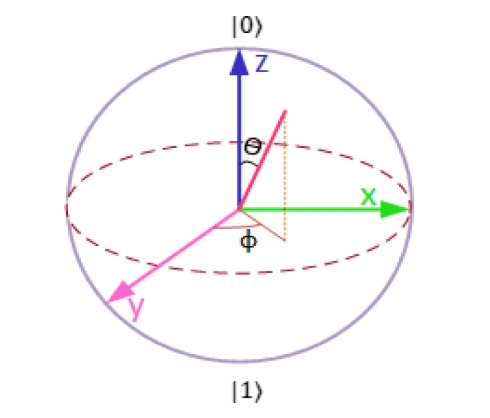
\includegraphics[width=.5\textwidth]{bloch.jpeg}}
\caption{بازنمایی کیوبیت در کره بلاچ}
\end{figure}

از آنجایی که یک پایان‌نامه یا رساله، یک نوشته بلند محسوب می‌شود، لذا اگر همه تنظیمات و مطالب پایان‌نامه را داخل یک فایل قرار بدهیم، باعث شلوغی
و سردرگمی می‌شود. به همین خاطر، قسمت‌های مختلف پایان‌نامه یا رساله  داخل فایل‌های جداگانه قرار گرفته است. مثلاً تنظیمات پایه‌ای کلاس، داخل فایل
\verb;AUTthesis.cls;، 
تنظیمات قابل تغییر توسط کاربر، داخل 
\verb;commands.tex;،
قسمت مشخصات فارسی پایان‌نامه، داخل 
\verb;fa_title.tex;,
مطالب فصل اول، داخل 
\verb;chapter1;
و ... قرار داده شده است. نکته مهمی که در اینجا وجود دارد این است که از بین این  فایل‌ها، فقط فایل 
\verb;AUTthesis.tex;
قابل اجرا است. یعنی بعد از تغییر فایل‌های دیگر، برای دیدن نتیجه تغییرات، باید این فایل را اجرا کرد. بقیه فایل‌ها به این فایل، کمک می‌کنند تا بتوانیم خروجی کار را ببینیم. اگر به فایل 
\verb;AUTthesis.tex;
دقت کنید، متوجه می‌شوید که قسمت‌های مختلف پایان‌نامه، توسط دستورهایی مانند 
\verb;input;
و
\verb;include;
به فایل اصلی، یعنی 
\verb;AUTthesis.tex;
معرفی شده‌اند. بنابراین، فایلی که همیشه با آن سروکار داریم، فایل 
\verb;AUTthesis.tex;
است.
در این فایل، فرض شده است که پایان‌نامه یا رساله شما، از5 فصل و یک پیوست، تشکیل شده است. با این حال، اگر
  پایان‌نامه یا رساله شما، بیشتر از 5 فصل و یک پیوست است، باید خودتان فصل‌های بیشتر را به این فایل، اضافه کنید. این کار، بسیار ساده است. فرض کنید بخواهید یک فصل دیگر هم به پایان‌نامه، اضافه کنید. برای این کار، کافی است یک فایل با نام 
\verb;chapter6;
و با پسوند 
\verb;.tex;
بسازید و آن را داخل پوشه 
\verb;AUTthesis;
قرار دهید و سپس این فایل را با دستور 
\texttt{\textbackslash include\{chapter6\}}
داخل فایل
\verb;AUTthesis.tex;
و بعد از دستور
\texttt{\textbackslash include\{chapter6\}}
 قرار دهید.

\section{نوع ناهنجاری}
قبل از هر چیز، بدیهی است که باید یک توزیع تِک مناسب مانند 
\verb;Live TeX;
و یک ویرایش‌گر تِک مانند
\verb;Texmaker;
را روی سیستم خود نصب کنید.  نسخه بهینه شده 
\verb;Texmaker;
را می‌توانید  از سایت 
 \href{http://www.parsilatex.com}{پارسی‌لاتک}%
\LTRfootnote{\url{http://www.parsilatex.com}}
 و
\verb;Live TeX;
را هم می‌توانید از 
 \href{http://www.tug.org/texlive}{سایت رسمی آن}%
\LTRfootnote{\url{http://www.tug.org/texlive}}
 دانلود کنید.
 
در مرحله بعد، سعی کنید که  یک پشتیبان از پوشه 
\verb;AUTthesis;
 بگیرید و آن را در یک جایی از هارددیسک سیستم خود ذخیره کنید تا در صورت خراب کردن فایل‌هایی که در حال حاضر، با آن‌ها کار می‌کنید، همه چیز را از 
 دست ندهید.
 
 حال اگر نوشتن پایان‌نامه اولین تجربه شما از کار با لاتک است، توصیه می‌شود که یک‌بار به طور سرسری، کتاب «%
\href{http://www.tug.ctan.org/tex-archive/info/lshort/persian/lshort.pdf}{مقدمه‌ای نه چندان کوتاه بر
\lr{\LaTeXe}}\LTRfootnote{\url{http://www.tug.ctan.org/tex-archive/info/lshort/persian/lshort.pdf}}»
   ترجمه دکتر مهدی امیدعلی، عضو هیات علمی دانشگاه شاهد را مطالعه کنید. این کتاب، کتاب بسیار کاملی است که خیلی از نیازهای شما در ارتباط با حروف‌چینی را برطرف می‌کند.
 
 
بعد از موارد گفته شده، فایل 
\verb;AUTthesis.tex;
و
\verb;fa_title;
را باز کنید و مشخصات پایان‌نامه خود مثل نام، نام خانوادگی، عنوان پایان‌نامه و ... را جایگزین مشخصات موجود در فایل
\verb;fa_title;
 کنید. دقت داشته باشید که نیازی نیست 
نگران چینش این مشخصات در فایل پی‌دی‌اف خروجی باشید. فایل 
\verb;AUTthesis.cls;
همه این کارها را به طور خودکار برای شما انجام می‌دهد. در ضمن، موقع تغییر دادن دستورهای داخل فایل
\verb;fa_title;
 کاملاً دقت کنید. این دستورها، خیلی حساس هستند و ممکن است با یک تغییر کوچک، موقع اجرا، خطا بگیرید. برای دیدن خروجی کار، فایل 
\verb;fa_title;
 را 
\verb;Save;، 
(نه 
\verb;As Save;)
کنید و بعد به فایل 
\verb;AUTthesis.tex;
برگشته و آن را اجرا کنید. حال اگر می‌خواهید مشخصات انگلیسی پایان‌نامه را هم عوض کنید، فایل 
\verb;en_title;
را باز کنید و مشخصات داخل آن را تغییر دهید.%
\RTLfootnote{
برای نوشتن پروژه کارشناسی، نیازی به وارد کردن مشخصات انگلیسی پروژه نیست. بنابراین، این مشخصات، به طور خودکار،
نادیده گرفته می‌شود.
}
 در اینجا هم برای دیدن خروجی، باید این فایل را 
\verb;Save;
کرده و بعد به فایل 
\verb;AUTthesis.tex;
برگشته و آن را اجرا کرد.

برای راحتی بیشتر، 
فایل 
\verb;AUTthesis.cls;
طوری طراحی شده است که کافی است فقط  یک‌بار مشخصات پایان‌نامه  را وارد کنید. هر جای دیگر که لازم به درج این مشخصات باشد، این مشخصات به طور خودکار درج می‌شود. با این حال، اگر مایل بودید، می‌توانید تنظیمات موجود را تغییر دهید. توجه داشته باشید که اگر کاربر مبتدی هستید و یا با ساختار فایل‌های  
\verb;cls;
 آشنایی ندارید، به هیچ وجه به این فایل، یعنی فایل 
\verb;AUTthesis.cls;
دست نزنید.

نکته دیگری که باید به آن توجه کنید این است که در فایل 
\verb;AUTthesis.cls;،
سه گزینه به نام‌های
\verb;bsc;,
\verb;msc;
و
\verb;phd;
برای تایپ پروژه، پایان‌نامه و رساله،
طراحی شده است. بنابراین اگر قصد تایپ پروژه کارشناسی، پایان‌نامه یا رساله را دارید، 
 در فایل 
\verb;AUTthesis.tex;
باید به ترتیب از گزینه‌های
\verb;bsc;،
\verb;msc;
و
\verb;phd;
استفاده کنید. با انتخاب هر کدام از این گزینه‌ها، تنظیمات مربوط به آنها به طور خودکار، اعمل می‌شود.

\section{ماهیت داده}
\subsection{انواع تصویربرداری}
همان‌طور که در بخش 
\ref{sec2}
گفته شد، برای جلوگیری از شلوغی و سردرگمی کاربر در هنگام حروف‌چینی، قسمت‌های مختلف پایان‌نامه از جمله فصل‌ها، در فایل‌های جداگانه‌ای قرار داده شده‌اند. 
بنابراین، اگر می‌خواهید مثلاً مطالب فصل ۱ را تایپ کنید، باید فایل‌های 
\verb;AUTthesis.tex;
و
\verb;chapter1;
را باز کنید و محتویات داخل فایل 
\verb;chapter1;
را پاک کرده و مطالب خود را تایپ کنید. توجه کنید که همان‌طور که قبلاً هم گفته شد، تنها فایل قابل اجرا، فایل 
\verb;AUTthesis.tex;
است. لذا برای دیدن حاصل (خروجی) فایل خود، باید فایل  
\verb;chapter1;
را 
\verb;Save;
کرده و سپس فایل 
\verb;AUTthesis.tex;
را اجرا کنید. یک نکته بدیهی که در اینجا وجود دارد، این است که لازم نیست که فصل‌های پایان‌نامه را به ترتیب تایپ کنید. می‌توانید ابتدا مطالب فصل ۳ را تایپ کنید و سپس مطالب فصل ۱ را تایپ کنید.

نکته بسیار مهمی که در اینجا باید گفته شود این است که سیستم
\lr{\TeX},
محتویات یک فایل تِک را به ترتیب پردازش می‌کند. به عنوان مثال، اگه فایلی، دارای ۴ خط دستور باشد، ابتدا خط ۱، بعد خط ۲، بعد خط ۳ و در آخر، خط ۴ پردازش می‌شود. بنابراین، اگر مثلاً مشغول تایپ مطالب فصل ۳ هستید، بهتر است
که دو دستور
\verb~\chapter{مقدمه}
بر اساس قانون مور
\LTRfootnote{Moore's law}
قدرت پردازنده های کامپیوتر های کلاسیک هر دو سال، دو برابر میشود. اما این رویه تا حدی ادامه خواهد داشت که محدودیت های دنیای فیزیک کلاسیک به آن اجازه دهند. چرا که اندازه ی اعضای تشکیل دهنده ی پردازنده ها به حدی کوچک میشود که ناخودآگاه وارد فضای کوچک کوانتوم
\LTRfootnote{Quantum}
 میشوند. پیشبینی میشود این اتفاق در سال 2050 رخ دهد.
\\
 پیچیدگی محاسباتی
\LTRfootnote{Computational complexity}
 برخی الگوریتم ها در کامپیوتر های کلاسیک کمتر قابلیت کاهش ندارند. در حالی که کامپیوتر های کوانتومی، در تئوری میتوانند با مقدار بزرگی داده همانند یک واحد داده برخورد کنند و پیچیدگی محاسباتی الگوریتم ها را کاهش دهند.
\cite{singhbook1in2}
به طور کلی، محاسبات کوانتومی از کنش و واکنش مواد در جهان در سطح ذرات تشکیل دهنده ی آن بهره میگیرد و بر روی بستر پدیده ی نسبیت خاص
\LTRfootnote{Special relativity}
 پایه‌گذاری شده‌است. 
\\
برای مثال، کامپیوتر کلاسیک مشکلی در پیدا کردن نام فرد موردنظر در یک کتاب تلفن ندارند. اما برای مسائل ریاضی بهینه سازی پیچیده
\LTRfootnote{Complex mathematical optimizing}
  که مسائلی هستند که برای پیدا کردن حالت بهینه با توجه به متغیر های مختلف است، کامپیوتر های کلاسیک پاسخگو نیستند. از جمله این مسائل میتوان به اختصاص دادن منابع در ساخت یک برج بزرگ برای بدست آوردن کمترین خرج ممکن اشاره کرد.  چنین مسائلی در همه ی خوزه ها وجود دارند و کامپیوتر های کوانتومی برای اجرای این الگوریتم ها بسیار مناسب هستند. 
\cite{singhbook1in4}

‌\section{‌خواص دنیای محاسبات کوانتومی}
\subsection{کیوبیت}
کیوبیت ها
\LTRfootnote{Qubits}
 در کامپیوتر های کوانتومی، معادل بیت ها
\LTRfootnote{bits}
 در کامپیوتر های کلاسیک هستند. یک بیت یا در حالت صفر قرار دارد یا در حالت یک قرار دارد. تفاوت کیوبیت ها در این است که میتوانند حالی به جز صفر یا یک داشته باشند یا میتوان گفت برهم‌نهی 
\LTRfootnote{superposition}
حالات را شاهد هستیم. درنتیجه، کیوبیت میتواند حالات بیشتری از بیت داشته باشد. هر کیوبیت، به یک احتمالی میتواند یک باشد و به یک احتمالی میتواند صفر باشد. 
\begin{equation}
\left|\Psi\right\rangle = \alpha\left|0\right\rangle + \beta\left|1\right\rangle = \begin{bmatrix}
 \alpha
\\
\beta
\end{bmatrix}
\end{equation}
به طوری که 
$\alpha$
 و 
$\beta$
  شدت احتمال هستند و هر دو اعداد مختلط هستند به طوری که
\begin{equation}
\alpha^{2} + \beta^{2} = 1
\end{equation}
فضای حالتی که این دو متغیر تشکیل میدهند، یک فضای مختلط دو بعدی است.  حالات خاص صفر و یک، یک فضای بردار پایه ای
\LTRfootnote{orthonormal basis}
برای این فضای برداری تشکیل میدهند.
\begin{equation}
\left|0\right\rangle = (0, 1) and \left|1\right\rangle = (1, 0)
\end{equation}
در شکل پایین، میتوانید کره ی بلاچ
\LTRfootnote{Bloch's sphere}
  که نوعی بازنمایی هندسی از حالت یک کیوبیت است، را مشاهده کنید.
\begin{figure}[!h]
\centerline{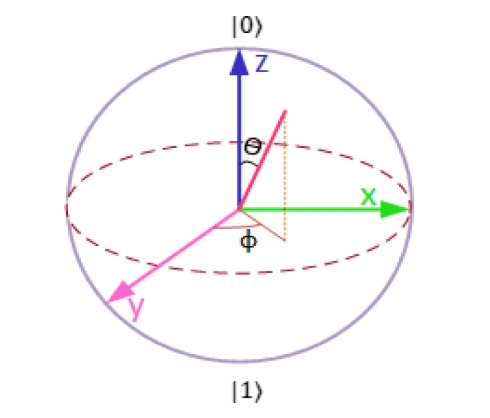
\includegraphics[width=.5\textwidth]{bloch.jpeg}}
\caption{بازنمایی کیوبیت در کره بلاچ}
\end{figure}
این بازنمایی را میتوانید به تعداد نامحدودی کیوبیت هم انطباق دهید. به طوری که با داشتن $n$ کیوبیت نیاز به نگهداری $n^{2}$ عدد خواهید داشت. این حالت زمانی رخ میدهد که $n$ کیوبیت درهم‌تنیده
\LTRfootnote{entangled}
 شوند به طوری که باهم یک حالت را تشکیل دهند و نتوان آن ها را جدا کرد. 
\cite{fundamentalsandapplications}
همچنان جمع مجذور همه ی مقادیر باید برابر با یک شود. نمایش انتزاعی دو کیوبیت به شکل زیر خواهد بود:
\begin{equation}
\left|\Psi\right\rangle = \alpha_{0}\left|00\right\rangle +  \alpha_{1}\left|01\right\rangle +  \alpha_{2}\left|10\right\rangle +  \alpha_{3}\left|11\right\rangle = \begin{bmatrix}
 \alpha_{0}
\\
 \alpha_{1}
\\
 \alpha_{2}
\\
 \alpha_{3}
\end{bmatrix}
\end{equation}
نمایش دو کیوبیت در فرم ماتریسی و دیراک
\LTRfootnote{Dirac}
:
\begin{equation}
\left|00\right\rangle  = \begin{bmatrix}
 \alpha_{1}
\\
 \alpha_{0}
\\
 \alpha_{0}
\\
 \alpha_{0}
\end{bmatrix}
\text{;}
\left|01\right\rangle  = \begin{bmatrix}
 \alpha_{0}
\\
 \alpha_{1}
\\
 \alpha_{0}
\\
 \alpha_{0}
\end{bmatrix}
\text{;}
\left|10\right\rangle  = \begin{bmatrix}
 \alpha_{0}
\\
 \alpha_{0}
\\
 \alpha_{1}
\\
 \alpha_{0}
\end{bmatrix}
\text{;}
\left|11\right\rangle  = \begin{bmatrix}
 \alpha_{0}
\\
 \alpha_{0}
\\
 \alpha_{0}
\\
 \alpha_{1}
\end{bmatrix}
\end{equation}


\subsection{ضرب تانسوری}
ضرب تانسوری
\LTRfootnote{Tensor product}
، عملیاتی است که بین دو ماتریس میتوان انجام داد. این عملیات، یکی از بخش های اصلی محاسبات کوانتومی است. برای اینکه بتوان سیستم های چند-کیوبیتی
\LTRfootnote{multiple-qubit systems}
را به صورت ریاضی نمایش داد، از این عملیات استفاده میشود. به این صورت که اگر $M$ یک ماتریس $(p,q)$ باشد و  $N$ یک ماتریس $(x,y)$ باشد، ماتریس ضرب تانسوری آنها یک ماتریس $(px,qy)$ خواهد بود. 
\cite{fundamentalsandapplications}
این ضرب را میتوان با یک گیت کوانتومی
\LTRfootnote{quantum gate}
 اعمال کرد.
\begin{equation}
M =  \begin{bmatrix}
 a_{11} &  a_{12}
\\
 a_{21} & a_{22}
\end{bmatrix}
\text{;}
N =  \begin{bmatrix}
 b_{11} &  b_{12}
\\
 b_{21} &  b_{22}
\end{bmatrix}
\end{equation}

\begin{equation}
M \oplus  N =  \begin{bmatrix}
 a_{11}b_{11} &  a_{11}b_{12} &  a_{12}b_{11} &  a_{12}b_{12}
\\
 a_{11}b_{21} &  a_{11}b_{22} &  a_{12}b_{21} &  a_{12}b_{22}
\\
 a_{21}b_{11} &  a_{21}b_{12} &  a_{22}b_{11} &  a_{22}b_{12}
\\
 a_{21}b_{21} &  a_{21}b_{22} &  a_{22}b_{21} &  a_{22}b_{22}
\end{bmatrix}
\end{equation}
برای ضرب تانسوری دو کیوبیت خواهیم داشت:
\begin{equation}
\left|0\right\rangle  \oplus  \left|1\right\rangle  =
\begin{bmatrix}
1 \\ 0 
\end{bmatrix} 
\oplus 
\begin{bmatrix}
0 \\ 1 
\end{bmatrix} 
=
  \begin{bmatrix}
0
\\
1
\\
0
\\
0
\end{bmatrix} = \left|01\right\rangle
\end{equation}
~
و
\verb~\chapter{طریقه‌ی مرجع نویسی و واژه‌نامه‌}
\section{طریقه‌ی مرجع نویسی}
برای نوشتن مراجع پایان نامه، برای راحتی کار به صورت زیر عمل می‌کنیم:
\subsection{بارگیری مراجع}
در ابتدا مراجع را باید از سایت‌های معتبر بارگیری کنیم، مثلا برای ارجاع دادن به مقاله‌ی
\lr{A classification of some Finsler connections and their applications}
ابتدا به سایت
\href{scholar.google.com}{گوگل اسکولار} 
رفته و این مقاله را جستجو می‌کنیم. پس از پیدا کردن این مقاله، مانند شکل زیر، در زیر نام و چکیده‌ی مقاله، $5$ گزینه وجود دارد که عبارتند از:\\

\begin{enumerate}
\item \lr{ Cited by}

\item \lr{ Related articles}

\item \lr{ All 6 versions}

\item \lr{ Cite}

\item \lr{ Save}
\end{enumerate}
\begin{figure}[!h]
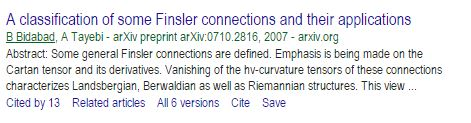
\includegraphics[height=3cm]{bidabad}
\caption{نمونه یک مقاله در گوگل اسکولار}
\end{figure}
در اینجا ما به گزینه‌ی چهارم یعنی
\lr{ Cite}
احتیاج داریم. بر روی آن کلیک کرده و پنجره‌ای مانند
\cref{fig.2}
باز می‌شود که دارای $4$ گزینه‌ی زیر است:
\begin{enumerate}
\item \lr{BibTeX}

\item \lr{EndNote}

\item \lr{RefMan}

\item \lr{RefWorks}
\end{enumerate}
\begin{figure}
\centering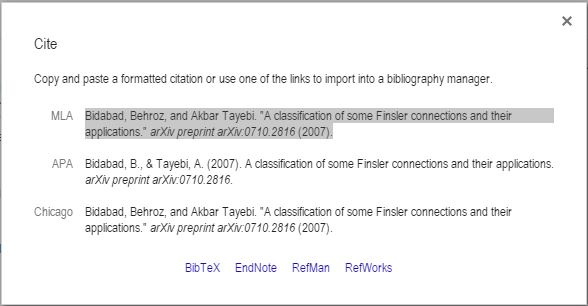
\includegraphics[scale=.6]{bibref}
\caption{پنجره‌ی باز شده در گوگل اسکولار}\label{fig.2}
\end{figure}
روی گزینه‌ی اول، یعنی
\verb;BibTeX;
کلیک کرده و همه‌ی نوشته‌های پنجره‌ی باز شده را مانند زیر، کپی کرده و در فایل
\verb;references.bib;
موجود در فایل
\verb;AUTthesis;
پیست می‌کنیم. سپس کلیدهای
\verb;Ctrl+s;
را می‌زنیم تا فایل ذخیره شود.\\
\begin{latin}
	\normalsize
\begin{verbatim}
@ article{bidabad2007classification,
title={A classification of some Finsler connections and their applications},
author={Bidabad, Behroz and Tayebi, Akbar},
journal={arXiv preprint arXiv:0710.2816},
year={2007}
}
\end{verbatim}
\end{latin}
\subsection{روش ارجاع در متن}
برای ارجاع دادن به مقاله‌ی بالا، باید در جایی که می‌خواهید ارجاع دهید، دستور زیر را تایپ کنید:
\begin{latin}
\lr{$\backslash$cite\{bidabad2007classification\}}
\end{latin}
همانطور که مشاهده می‌کنید از کلمه‌ای که در سطر اول ادرس مقاله آمده (یعنی کلمه‌ی پس از
\lr{@article$\lbrace$})
استفاده کرده‌ایم. پس از دستور فوق، به صورت \cite{bidabad2007classification} و \cite{aa} مرجع خواهد خورد. توجه شود که در صورتی مراجع چاپ خواهند شد که در متن به انها ارجاع داده شده باشد. همچنین برای ارجاع چندتایی از دستور 
\lr{$\backslash$cite\{name1, name2,...\}}
استفاده کنید که به‌صورت \cite{najafi2008finsler, zakeri, najafi} ارجاع خواهند خورد.
\subsection{روش اجرای برنامه}
ابتدا فایل
\verb;AUT_thesis.tex;
را باز کرده و آن را دو بار اجرا کنید. سپس حالت اجرا را از 
\verb;Build Quick;
به حالت
\verb;Bibtex;
تغییر داده و دوباره برنامه را اجرا کنید. دو بار دیگر برنامه را در حالت 
\verb;Build Quick;
اجرا کرده و نتیجه را مشاهده کنید. در این روش تمامی مراجع بر اساس اینکه کدام یک در متن زودتر به آن ارجع داده شده لیست خواهند شد.
\subsection{مراجع فارسی}
برای نوشتن مراجع فارسی باید به صورت دستی، در همان فایل قبلی به صورت زیر عمل می‌کنیم:
\begin{LTR}
\noindent\verb;@article{manifold,;\\
\verb;title={;منیفلد هندسه\verb;},;\\
\verb;author={;بیدآباد دکتربهروز \verb;},;\\
\verb;journal{; امیرکبیر صنعتی دانشگاه\verb;},;\\
\verb;year={1389},;\\
\verb;LANGUAGE={Persian};\\
\verb;};
\end{LTR}
همانطور که مشاهده می‌کنید تنها تفاوت آن با حالت مراجع انگلیسی، سطر آخر آن می‌باشد که زبان را مشخص می‌کند که حتماً باید نوشته شود.
\section{راهنمای واژه‌نامه}

به دلیل پیچیدگی واژه‌نامه‌های موجود در سایت پارسی لاتک، از روش زیر برای نوشتن واژه‌نامه استفاده کنید:

ابتدا با استفاده از اکسل، واژه های خود را یک‌بار براساس حروف الفبای فرسی و بار دیگر انگلیسی مرتب کنید. سپس واژه ها را در فایل \lr{dicen2fa} و \lr{dicfa2en} قرار دهید.

\section{ساخت نمایه}\label{Namaye}
\subsection{ساخت نمایه}
 \begin{enumerate}

\item
کلمات مورد نظر خود مثلا \lr{word} با دستور \verb|\index{word}| ایندکس کنید.
\item
نحوه‌ی اجرای \lr{Make Index}   در ویرایشگرهای \lr{TeX Maker} و \lr{TeX Works}:
\begin{itemize}
\item  تک‌میکر: از منوی \lr{Tools} گزینه‌ی \lr{Xindy Make Index} را کلیک کنید یا از دکمه‌‌های میانبر \lr{Ctrl+Alt+I} استفاده کنید.

\item  تک‌ورکز: ابتدا باید مثل عکس زیر تنظیم  و سپس گزینه‌ی \lr{Xindy Make Index}  انتخاب و روی دکمه‌ی سبز رنگ کلیک کنید یا از دکمه‌های  \lr{Ctrl+T} استفاده کنید.

\begin{figure}[!h]
\centerline{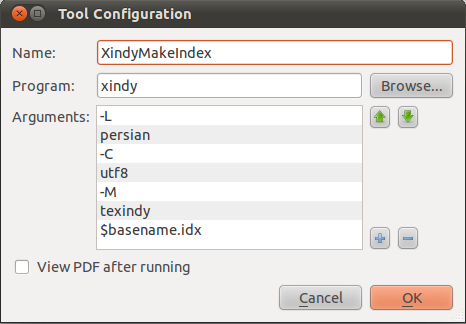
\includegraphics[width=.5\textwidth]{Xindy_Make_Index.png}}
\caption{تنظیمات مربوط به تک‌ورکز}
\end{figure}

\end{itemize}
 \end{enumerate}
 
 \index{کتاب}
\index{پارسی‌لاتک}
\index{بی‌دی}
\index{سوال}
\index{عنصر}
\index{گزینه}
\index{ژاکت}
\index{مرکز دانلود}
\index{اجرا}
\index{تک‌لایو}
\index{ثالث}
\index{جهان}
\index{چهار}
\index{حمایت}
\index{خواهش}
\index{دنیا}
\index{زی‌پرشین}
\index{ریحان}
\index{شیرین}
\index{صمیمی}
\index{ضمیر}
\index{طبیب}~
را در فایل 
\verb~AUTthesis.tex~،
غیرفعال%
\RTLfootnote{
برای غیرفعال کردن یک دستور، کافی است پشت آن، یک علامت
\%
 بگذارید.
}
 کنید. زیرا در غیر این صورت، ابتدا مطالب فصل ۱ و ۲ پردازش شده (که به درد ما نمی‌خورد؛ چون ما می‌خواهیم خروجی فصل ۳ را ببینیم) و سپس مطالب فصل ۳ پردازش می‌شود و این کار باعث طولانی شدن زمان اجرا می‌شود. زیرا هر چقدر حجم فایل اجرا شده، بیشتر باشد، زمان بیشتری هم برای اجرای آن، صرف می‌شود.

\subsection{انواع فرمت های تصویر}
برای وارد کردن مراجع به فصل 2
مراجعه کنید.
\subsection{آسیب های ممکن}
برای وارد کردن واژه‌نامه فارسی به انگلیسی و برعکس، بهتر است مانند روش بکار رفته در فایل‌های 
\verb;dicfa2en;
و
\verb;dicen2fa;
عمل کنید.
\nocite{*}
\section{انتخاب روش نهایی}
برای پرسیدن سوال‌های خود در مورد حروف‌چینی با زی‌پرشین،  می‌توانید به
 \href{http://forum.parsilatex.com}{تالار گفتگوی پارسی‌لاتک}%
\LTRfootnote{\url{http://www.forum.parsilatex.com}}
مراجعه کنید. شما هم می‌توانید روزی به سوال‌های دیگران در این تالار، جواب بدهید.
